

\documentclass{article}

% Packages

\usepackage[margin=1in]{geometry}
%\usepackage{graphicx}
%\usepackage{tikz-timing}
\usepackage{color}
\usepackage{commath}

\usepackage{setspace}
\doublespacing

\usepackage{cite}
\usepackage{caption}
\usepackage{subcaption}
\usepackage{hyperref}

% Automatix LaTeX build system modules

%\usepackage{svg}
%\usepackage{mat}
\usepackage[dvipdfm]{graphicx} 
\usepackage{bmpsize}

%[stevo]: specify location of images here
%\usepackage{graphicx}
% declare the path(s) where your graphic files are
\graphicspath{{images/}}
% and their extensions so you won't have to specify these with
% every instance of \includegraphics
\DeclareGraphicsExtensions{.pdf,.jpeg,.png}

\newcommand{\degree}{\ensuremath{^\circ}}
% Now we actually start the document

\begin{document}

% Note that we are defining both the title and the author -- LaTeX will decide where
% they ought to go in the final typeset, depending on the style we've selected.

\title{ASTRO 121: Lab 3  \\ \normalsize Radio Interferometry at X Band}

\author{Rachel Hochman}


% The \markboth command simply determines how the pages will be marked.
% There are two arguments, since for double-sided pages, you often want a different
% marking on facing pages.

%\markboth{Team DarkStar, ASTRO121, Spring 2015}{Team DarkStar, ASTRO121, Spring 2015}

%Now we tell Latex to create the title, based on the info we've provided.

\maketitle


\section{Introduction}

The first goal of this lab was to learn about 'fringes.' We first explored how diffraction theory applies to an actual radio interferometer, and what the resulting fringe looks like in terms of its amplitude and phase. Once we obtained the fringe, we explored its properties further by taking a Fourier transform and Fourier filtering the fringe. We practiced these techniques on data taken of the Sun, and then we also obtained data of the Moon and a point source- W43 in our case. The other main goal of this lab was to expand on our knowledge of least-squares fitting techniques, specifically learning how to do \textit{nonlinear} least-squares fitting. Finally, we explored the Fourier transform relationship between interferometer response and sky brightness by using nonlinear least-squares fitting to obtain accurate diameters for the Sun and Moon.

\section{Experimental Setup}

All data collection for this lab was done with a multiplying interferometer.  The interferometer consists of two receiver dishes, each with a series of filters and mixers, as shown in \autoref{fig:interf}.  The received signal goes through a low power amplifier, a bandpass filter, a low noise amplifier, and a mixer within the feed of the dish. The signal is then brought into the lab where it goes through second bandpass filter, the second mixer, and a third bandpass filter. Finally the two signals from each side are mixed together in a DSB mixer.

An interferometer is desired over a single radio antenna because of increased angular resolution. Whereas the angular resolution of a single antenna with diameter \textit{D} is proportional to $\lambda/D$, the angular resolution achieved by two dishes separated by a baseline \textit{B} is proportional to $\lambda/B$. Consequently, the farther the two dishes are separated, the better the angular resolution.

\begin{figure}[h!]
 \begin{center}
    \includegraphics[width=5in, angle=90]{interf.ps}
    \caption{\bf{Interferometer Diagram}}
    \label{fig:interf}
     \end{center}
    \end{figure}
\newpage

The output of the interferometer is a sinusoidal-like signal called the "fringe."  Given a known baseline \textit{$B_y$} and the frequency, phase, and amplitude properties of the fringe, we can measure the declination of a point source as well as the diameters of the Sun and Moon. Exactly how will be discussed in later sections.

\subsection{Choosing an Observing Frequency}

There were some issues figuring this out...***TODO

\section{The Fringe}
Because we use two different dishes separated by baseline \textit{$B_y$}, there is a difference in their distances from the source. This difference is distance is made up of the geometrical path delay $\tau_{g}$ as well as any difference in cable length $\tau_{c}$. We know $\tau_{g}$, which is a function of the hour angle of the source ($h_s$), from the geometry of the interferometer. For the east-west baseline we have

\singlespacing
\begin{eqnarray}
 \tau_{g}(h_s) =\bigg[ \frac{B_y}{c}cos\;\delta \bigg] sin\;h_s
\end{eqnarray}

Therefore, the voltages for the two telescopes looking at a monochromatic source are: 

%\singlespacing
\begin{eqnarray}
 E_1(t) =cos(2\pi\nu t) \\
 E_2(t) =cos(2\pi\nu \big[ t+\tau_{tot}\big])
\end{eqnarray}
%\doublespacing

and the product is the interferometer fringe output:

\begin{eqnarray}
 F(t) =cos(2\pi\nu t) cos(2\pi\nu \big[ t+\tau_{tot}\big])
\end{eqnarray}
\doublespacing
Using various trig identities and the fact that $\frac{\nu}{c} = \lambda$ (see handout for each individual step) we are left with the fringe amplitude for a point source:


\begin{eqnarray}
 F(h_s) =Acos\bigg[ 2\pi(\frac{B_y}{c}cos\;\delta)sin\;h_s \bigg] -Bsin\bigg[ 2\pi(\frac{B_y}{c}cos\;\delta)sin\;h_s \bigg]
\end{eqnarray}

where  $A = cos(2\pi\nu\tau_c)$ and $B = sin(2\pi\nu\tau_c)$. Looking at the argument inside the cosine and sine in each term, we see a constant $C = \bigg[2\pi( \frac{B_y}{c}cos\;\delta )\bigg]$ multiplied by $sin(h_s)$. Because $h_s$ is the hour angle and increases monotonically with time, we can regard it as time. Therefore, the product $C sin(h_s)$ is the argument of the cosine terms and makes it oscillate with a with a frequency that depends on time. 

If you expand the hour angle term $sin(h_s)$ into a Taylor series, and consider that $F(h)$ varies as $f_f \;\Delta h$, you end up with a local fringe frequency of:

\begin{eqnarray}
f_f = \frac{C}{2\pi}cos(h_s)= \bigg(\frac{B_y}{\lambda}cos\delta \bigg) cos(h_s)
\label{eq:ff}
\end{eqnarray}
This value is in cycles per radian on the sky. To convert into cycles per minute, you must multiply by $\frac{2\pi}{60\times24}$ and to get cycles per second by $\frac{2\pi}{60\times60\times24}$.

\section{The Sun}
 
We began by taking fringe data of the Sun. A valuable exercise was to use the above 'local fringe frequency' equation to predict what frequencies we would see in the sun data, and then to confirm this by taking a Fourier transform of the Sun data. Our first set of Sun data was taken between the hour angles of -3 and 0. Therefore the values of $cos(h_s)$ should range from .707-1. Therefore, given a $B_y$ of 50ft and a $\lambda$ of 2.44 cm and substituting into \autoref{eq:ff} we expect to see a range of frequencies


\begin{figure}[h!]
 \begin{center}
    \includegraphics[width=6.5in]{sun_dft.ps}
    \caption{\bf{Sun DFT}}
    \label{fig:sun_dft}
     \end{center}
    \end{figure}
%%fig here of system
%
%%histogram plots here
%
%In order to check that our picosampler is set to the correct voltage threshold, we plotted a histogram of the data using the built in IDL function \texttt{histogram}. In \autoref{fig:histplots}, the histograms of the data gathered with the picosampler threshold set to 1V and 100mV are compared. 100mV is clearly the better choice since the data is not too quantized (as in the first plot) and looks like the well known Gaussian function.
%
%
%\begin{figure}[h!]
% \begin{center}
%    \includegraphics[width=4.5in]{histograms.ps}
%    \caption{\bf{Data Histogram Plots}}
%    \label{fig:histplots}
%     \end{center}
%    \end{figure}
%
%\subsection{Finding the Shape of the HI Line}
%
%We took data with two different mixing frequencies to obtain our 'online' and 'offline' spectra. We chose 1229.4 and 1231.4 as the two different initial LO frequencies in order to place the line in the middle of the upper sideband and the middle of the lower sideband, respectively. In \autoref{fig:avgplots} the effects of averaging the 'online' spectra and taking the median of the 'online' spectra are compared, along with the effects of smoothing the spectrum in the third plot.
%
%\begin{figure}[h!]
% \begin{center}
%    \includegraphics[width=5in]{avgvmedian.ps}
%    \caption{\bf{Averaging, Median, and Smoothing Effects}}
%    \label{fig:avgplots}
%     \end{center}
%    \end{figure}
%    
%    
%\newpage    
%    
%For comparison, the 'offline' spectrum is shown in \autoref{fig:offline}.
%
%\begin{figure}[h!]
% \begin{center}
%    \includegraphics[width=7in]{offline.ps}
%    \caption{\bf{Offline Spectrum}}
%    \label{fig:offline}
%     \end{center}
%    \end{figure}
%    
%    
%Once we have both the online and offline spectra, we can remove the instrumental bandpass to get the shape of the line by taking the ratio of the two. The ratios of $s_{online}/s_{offline}$ and  $s_{offline}/s_{online}$ are seen in \autoref{fig:ratio}.
%
%\begin{figure}[h!]
% \begin{center}
%    \includegraphics[width=6in]{ratio.ps}
%    \caption{\bf{Ratio of Spectra Giving the Shape of the Line}}
%    \label{fig:ratio}
%     \end{center}
%    \end{figure}
%    
% \subsection{Calibrating for Intensity}
% 
% In order to get the line intensity in terms of the calibration noise source, we took data with the horn looking at a cold sky, giving us $s_{coldsky}$ and with a human (Mahrud) acting as a blackbody to give us a spectrum, $s_{300K}$. We can obtain the scaling factor $T_{sys}$ by the following equation:
% 
%\begin{eqnarray}
%T_{sys} = \frac{\sum s_{coldsky}}{\sum (s_{300K}-s_{coldsky})}*T_{cal}
%\end{eqnarray}
%   
%Where $T_{cal}$ = 300K because that is the thermal power we injected by having Mahrud stand in front of the horn. Our calculated value for $T_{sys}$ is 266.4K.
%
%The final calibrated spectrum is given by $ratio \times T_{sys}$. The plot in \autoref{fig:finalcal} was obtained by taking the spectra of each ratio and averaging them, then plotting vs RF frequency.
%
% \begin{figure}[h!]
% \begin{center}
%    \includegraphics[width=6in]{finalcalspec.ps}
%    \caption{\bf{Final Calibrated Spectrum vs RF Frequency}}
%    \label{fig:finalcal}
%     \end{center}
%    \end{figure}
%\newpage
%   
%\subsection{Corrections for Doppler Velocity}    
%    
%In addition, I have plotted the final calibrated spectrum vs Doppler Velocity. The velocity values were calculated based on the Doppler formula:
%    
% \begin{eqnarray}
% \frac{v}{c} =- \frac{\Delta f}{f_{0}}
%\end{eqnarray}   
%    
% \begin{figure}[h!]
% \begin{center}
%    \includegraphics[width=6in]{finalcalVEL.ps}
%    \caption{\bf{Final Calibrated Spectrum vs Doppler Velocity}}
%    \label{fig:finalcalvel}
%     \end{center}
%    \end{figure}
%   
% Finally, we need to correct the observed velocity for the orbital velocity and spin of the Earth. Here we have used the \texttt{ugdoppler.pro} procedure to correct the velocities and express them with respect to the Local Standard of Rest (LSR) and the Barycentric (Sun) reference frames. In \autoref{fig:corrvel}, the velocity with respect to the Barycentric frame is above and the LSR frame is below. Note, they only differ by a few km/s. The values have been calculated using the following values.
% 
%\texttt{ \\
%lat = 37.873 \\
%lng = -122.257 \\
%tzone = 8 \\
%juliandate = 2457071.50603\\
%\\
%\\
%\\} 
%    
%     \begin{figure}[h!]
% \begin{center}
%    \includegraphics[width=6in]{corr_vel.ps}
%    \caption{\bf{Final Calibrated Spectrum vs Corrected Doppler Velocity}}
%    \label{fig:corrvel}
%     \end{center}
%    \end{figure}
%
%\newpage
%
%\section{VSWR Measurement}
%When transferring power using electromagnetic waves moving through a medium such as cables or waveguides, it is not necessarily the case that all of the input power is transmitted when there is a change in medium. In real systems, if the impedance is different on either side, part of the power is reflected back towards the source. This condition is known as impedance mismatch. 
%The voltage reflection coefficient for a load with resistance $R_L$ that terminates a line with impedance $Z_0$ is 
%
%\begin{eqnarray}
%\rho = \frac{V_R}{V_F}=\frac{R_L - Z_0}{R_L+Z_0}
%\end{eqnarray}
%
%Where $V_R$ is the reflected voltage amplitude and $V_F$ the forward one. The reflected voltage will interfere with the forward wave constructively and destructively, creating peaks and valleys in the voltage at different distances on the first medium.  The Voltage Standing Wave Ratio, or VSWR, is the ratio of $V_{max}$, the maximum voltage created by constructive interference, over $V_{min}$, the minimum voltage created by destructive interference throughout the medium:
%
%\begin{eqnarray}
%VSWR = \frac{|V_{max}|}{|V_{min}|}=\frac{1+\rho}{1-\rho}
%\end{eqnarray}
%
%
%\subsection{Standing Waves in Coax Cable}
%
%One of the most effective methods of transmitting radio frequency signals is via coaxial cables. In a coax cable a conductive outer layer is grounded and wrapped around the signal carrying core with a dielectric insulator between the core and the shield. The advantage of this design is that electric and magnetic fields are confined to the dielectric with little leakage. In addition, electric and magnetic fields outside the cable are kept from causing interference with the signal on the core.
%
%In order to measure VSWR in coax cables we use a slotted coax cable with a probe that can measure the electric field inside the dielectric. The probe is connected to a radio detector which converts electromagnetic waves to a voltage that we can read on a voltmeter. We connect one end of the cable to a signal generator set at 3GHz and leave the other end open. Since the impedance inside the cable (50�) does not match the impedance of free space (infinite), the power will be reflected and we should expect to see standing waves. %\autoref{fig:cabledata} shows the measurements of the nulls and zeros.
%
%
%Taking a simple average of the values between zeros gives us a $\lambda /2$ of 50.1mm. However, using a least squares method (as described below), I find that the wave has a $\lambda /2$ of 49.8515mm. Therefore the wavelength is .0997 m. Using the formula $\lambda\upsilon = c$, that gives a velocity of $.0997  \times 3e9 =  2.991e8\: m/s$ through the coaxial cable, which is roughly the speed of light as we would expect. Note that using the simple averaging method would have given a velocity just greater that the speed of light!
%
%The least squares matrix method was done in Matlab as follows:
%
% \texttt{\\
% \%input in the form of a matrix, rows contain points \\
% x=[1,520;2,1020;3,1530;4,2035;5,2535;6,3040;7,3510;8,4025;9,4505;10,5015]                    \\
% \%forming A of Ax=b \\
% a=[1,x(1,1);1,x(2,1);1,x(3,1);1,x(4,1);1,x(5,1);1,x(6,1);1,x(7,1);1,x(8,1);1,x(9,1);1,x(10,1)]           \\
% \%forming b of Ax=b \\
% b=[x(1,2);x(2,2);x(3,2);x(4,2);x(5,2);x(6,2);x(7,2);x(8,2);x(9,2);x(10,2)]                \\
% \%computing projection of matrix A on b, giving x \\
% yy=inv(transpose(a)*a)*transpose(a)*b }
%
%
%
%When the coax cable is terminated with a matched load, the wave is not reflected and therefore there is roughly no standing wave in the cable.
%
%
%
%\subsection{Standing Waves in X-Band Waveguide}
%
%We repeated similar measurements with an X-Band Waveguide, taking standing wave measurements for both the open ended and shorted opening cases. The wavelengths in the table below were calculated using a least squares approach. 
%
%
%\begin{table}[h!]
%\renewcommand{\arraystretch}{1.1}
%
%\label{Wavelengths}
%\centering
%\begin{tabular}{|c|c|c|c|c|}
%
%\hline
%\bf{Input Frequency}		&\bf{Open $\lambda$(cm)}	&\bf{Open Velocity (Gm/s)}	&\bf{Closed $\lambda$(cm)} &\bf{Closed Velocity(Gm/s)}\\
%
%\hline  
%
%
%7.5GHz	&8.26	&.6195& 7.972&.5979\\
%\hline
%
%
%
%7.75GHz	&7.436 &.57629&7.336&.56854\\	
%\hline
%
%
%8GHz	&6.4756 &.51804&6.5612&.52489\\
%\hline
%
%8.25GHz &6.132 &.50589&6.0412&.49839\\
%\hline
%
%8.5GHz &5.5644&.47297 &5.5756 &.47393\\
%\hline
%
%8.75GHz &5.2016&.45514 &5.11&.44713\\
%\hline
%
%\end{tabular}
%\caption{\bf{Wavelengths and Velocities in the Waveguide}}
%\end{table}
%
%
%But wait, one might say- the velocities calculated above are fast than the speed of light! This becomes less puzzling when we realize that what we are actually measuring is the 'phase velocity' given by $\upsilon_{p} = \frac{c}{sin \theta}$. Just like waves in the ocean, because a line of constant phase is perpendicular to the direction in which the wave is traveling, the phase velocity along the 'beach' is faster than 3e8.
%
%Finally, we are able to derive the cutoff wavelength of this particular waveguide by extrapolating from the data we measured. We already know that the cutoff frequency s 7GHz, and as seen in \autoref{fig:wv}, the line of best fit extended back to 7GHZ gives us a wavelength of approximately 9cm.
%
% \begin{figure}[h!]
% \begin{center}
%    \includegraphics[width=5in]{figure_1.ps}
%    \caption{\bf{Wavelengths with Line of Best Fit (Plot by Stevo)}}
%    \label{fig:wv}
%     \end{center}
%    \end{figure}
%
%\section{Conclusion}
%In this lab we found the shape of the 21-cm line from atomic Hydrogen in our galaxy and calibrated the results to remove the instrumental contribution to the spectrum. In the second part of the lab we learned about reflections and impedance matching, VSWR, and how to derive cable lengths and propagation velocities by measuring reflections and wavelengths in both coax cables and waveguides. Lastly, we used linear least-squares fitting to get the most accurate results from our data. 
%
%\section{Acknowledgements and Notes}
%Thanks to Professor Carl Heiles and Katherine DeKleer for their help. Thanks also to the other members of Team Darkstar: Stevo Bailey, Brianna Grado-White, and Mahrud Sayrafi. Thanks this week to team CRAM, for sharing their waveguide raw data with us.
%





\end{document}


--------------------------------------------------------------------------------
